
%% bare_conf_compsoc.tex
%% V1.4b
%% 2015/08/26
%% by Michael Shell
%% See:
%% http://www.michaelshell.org/
%% for current contact information.
%%
%% This is a skeleton file demonstrating the use of IEEEtran.cls
%% (requires IEEEtran.cls version 1.8b or later) with an IEEE Computer
%% Society conference paper.
%%
%% Support sites:
%% http://www.michaelshell.org/tex/ieeetran/
%% http://www.ctan.org/pkg/ieeetran
%% and
%% http://www.ieee.org/

%%*************************************************************************
%% Legal Notice:
%% This code is offered as-is without any warranty either expressed or
%% implied; without even the implied warranty of MERCHANTABILITY or
%% FITNESS FOR A PARTICULAR PURPOSE! 
%% User assumes all risk.
%% In no event shall the IEEE or any contributor to this code be liable for
%% any damages or losses, including, but not limited to, incidental,
%% consequential, or any other damages, resulting from the use or misuse
%% of any information contained here.
%%
%% All comments are the opinions of their respective authors and are not
%% necessarily endorsed by the IEEE.
%%
%% This work is distributed under the LaTeX Project Public License (LPPL)
%% ( http://www.latex-project.org/ ) version 1.3, and may be freely used,
%% distributed and modified. A copy of the LPPL, version 1.3, is included
%% in the base LaTeX documentation of all distributions of LaTeX released
%% 2003/12/01 or later.
%% Retain all contribution notices and credits.
%% ** Modified files should be clearly indicated as such, including  **
%% ** renaming them and changing author support contact information. **
%%*************************************************************************


% *** Authors should verify (and, if needed, correct) their LaTeX system  ***
% *** with the testflow diagnostic prior to trusting their LaTeX platform ***
% *** with production work. The IEEE's font choices and paper sizes can   ***
% *** trigger bugs that do not appear when using other class files.       ***                          ***
% The testflow support page is at:
% http://www.michaelshell.org/tex/testflow/

\documentclass[conference,compsoc]{IEEEtran}
% Some/most Computer Society conferences require the compsoc mode option,
% but others may want the standard conference format.
%
% If IEEEtran.cls has not been installed into the LaTeX system files,
% manually specify the path to it like:
% \documentclass[conference,compsoc]{../sty/IEEEtran}


% Some very useful LaTeX packages include:
% (uncomment the ones you want to load)

% *** MISC UTILITY PACKAGES ***
\usepackage{textcomp}
\usepackage[usenames,dvipsnames,svgnames,table]{xcolor}
\usepackage[utf8]{inputenc}
\usepackage{amssymb}
\usepackage{pifont}
\newcommand{\cmark}{\ding{51}}
\newcommand{\xmark}{\ding{55}}
\newcommand{\wavedash}{\ding{83}}

% sol macros
\newcommand{\loungecxx}{Lounge\textless{}C++\textgreater{}}
\newcommand{\soltwo}{Sol\textsuperscript{2}}

% lots of stuff just to get basic unicode stuff...
\DeclareUnicodeCharacter{2714}{\cmark{}}
\DeclareUnicodeCharacter{2717}{\xmark{}}
\DeclareUnicodeCharacter{301C}{\wavedash{}}
%\usepackage{ifpdf}
% Heiko Oberdiek's ifpdf.sty is very useful if you need conditional
% compilation based on whether the output is pdf or dvi.
% usage:
% \ifpdf
%   % pdf code
% \else
%   % dvi code
% \fi
% The latest version of ifpdf.sty can be obtained from:
% http://www.ctan.org/pkg/ifpdf
% Also, note that IEEEtran.cls V1.7 and later provides a builtin
% \ifCLASSINFOpdf conditional that works the same way.
% When switching from latex to pdflatex and vice-versa, the compiler may
% have to be run twice to clear warning/error messages.
\usepackage{listings}

% *** IN-PAPER REFERENCES ***
\usepackage{hyperref}
\usepackage{cleveref}
\hypersetup{
	colorlinks=true, 
	linkcolor=Violet,
	citecolor=Periwinkle,
	filecolor=magenta,
	urlcolor=ForestGreen
}
\crefname{section}{§}{§§}
\Crefname{Section}{§}{§§}
\crefname{listing}{snippet}{snippet}
\Crefname{listing}{Snippet}{Snippet}
% clever references


% *** LISTING STYLES ***

\definecolor{cxxlistingbackground}{rgb}{0.97,0.97,0.97}
\definecolor{NearBlack}{rgb}{0.15,0.15,0.15}

\lstset{
	backgroundcolor=\color{cxxlistingbackground},
	tabsize=5,
	language=C++,
	captionpos=b,
	numbers=left,
	numberstyle=\tiny,
	numbersep=5pt,
	breaklines=true,
	showstringspaces=false,
	basicstyle=\footnotesize,
	keywordstyle=\color{RoyalPurple},
	commentstyle=\color{DarkGreen},
	stringstyle=\color{RawSienna},
	identifierstyle=\color{NearBlack},
	xleftmargin=0.5cm,
	frame=lr,
	framesep=8pt,
	framerule=0pt,
	%frame=lines,
	% use emph list for some additional keywords
	emph={
		basic,
		SLB, Script, Manager,
		sel, Selector,
		sol, luwra, function, protected_function, table, usertype, coroutine, userdata, lightuserdata, thread, reference, state, state_view, variadic_args, this_state, nil,
		kaguya, State, Function, Thread, Table,
		std, string, tuple, map, experimental, optional,
		LuaIntf, LuaTable, LuaContext, LuaBinding
		luwra,
		luabind, class_, constructor,
		lua_State,
		LUAPP_USERDATA,
		OOLUA, OOLUA_PROXY, OOLUA_PROXY_END, OOLUA_MGET_MSET, OOLUA_MGET_MSET, OOLUA_MFUNC, OOLUA_MFUNC_CONST, OOLUA_EXPORT_FUNCTIONS_CONST, OOLUA_EXPORT_FUNCTIONS, OOLUA_FUNC, OOLUA_CFUNC,
	},
	emphstyle={\color{NavyBlue}},
	ndkeywords={
		luaL_newstate, luaL_openlibs, luaL_dostring, lua_error,
		open, module, def, def_nonconst, def_const, def_readwrite,
		writeVariable, readVariable,
		beginClass, addConstructor, addFunction, addVariable, endClass,
		multi_return, basic_call, get, set, basic_multi_param,
		push, pop, check, check_get,
		foo, bar, baz, qux,
	},
	ndkeywordstyle=\color{WildStrawberry},
}
\renewcommand{\lstlistingname}{Snippet}
\renewcommand{\lstlistlistingname}{List of \lstlistingname s}

\newcommand\digitstyle{\color{WildStrawberry}}
\makeatletter
\newcommand{\ProcessDigit}[1]
{%
	\ifnum\lst@mode=\lst@Pmode\relax%
	{\digitstyle #1}%
	\else
	#1%
	\fi
}
\makeatother
\lstset{literate=
	{0}{{{\ProcessDigit{0}}}}1
	{1}{{{\ProcessDigit{1}}}}1
	{2}{{{\ProcessDigit{2}}}}1
	{3}{{{\ProcessDigit{3}}}}1
	{4}{{{\ProcessDigit{4}}}}1
	{5}{{{\ProcessDigit{5}}}}1
	{6}{{{\ProcessDigit{6}}}}1
	{7}{{{\ProcessDigit{7}}}}1
	{8}{{{\ProcessDigit{8}}}}1
	{9}{{{\ProcessDigit{9}}}}1
	{<=}{{\(\leq\)}}1,
	morestring=[b]",
	morestring=[b]',
	morecomment=[l]//,
}


% *** CITATION PACKAGES ***
%
\ifCLASSOPTIONcompsoc
  % IEEE Computer Society needs nocompress option
  % requires cite.sty v4.0 or later (November 2003)
  \usepackage[nocompress]{cite}
\else
  % normal IEEE
  \usepackage{cite}
\fi
% cite.sty was written by Donald Arseneau
% V1.6 and later of IEEEtran pre-defines the format of the cite.sty package
% \cite{} output to follow that of the IEEE. Loading the cite package will
% result in citation numbers being automatically sorted and properly
% "compressed/ranged". e.g., [1], [9], [2], [7], [5], [6] without using
% cite.sty will become [1], [2], [5]--[7], [9] using cite.sty. cite.sty's
% \cite will automatically add leading space, if needed. Use cite.sty's
% noadjust option (cite.sty V3.8 and later) if you want to turn this off
% such as if a citation ever needs to be enclosed in parenthesis.
% cite.sty is already installed on most LaTeX systems. Be sure and use
% version 5.0 (2009-03-20) and later if using hyperref.sty.
% The latest version can be obtained at:
% http://www.ctan.org/pkg/cite
% The documentation is contained in the cite.sty file itself.
%
% Note that some packages require special options to format as the Computer
% Society requires. In particular, Computer Society  papers do not use
% compressed citation ranges as is done in typical IEEE papers
% (e.g., [1]-[4]). Instead, they list every citation separately in order
% (e.g., [1], [2], [3], [4]). To get the latter we need to load the cite
% package with the nocompress option which is supported by cite.sty v4.0
% and later.





% *** GRAPHICS RELATED PACKAGES ***
%
\ifCLASSINFOpdf
  \usepackage[pdftex]{graphicx}
  % declare the path(s) where your graphic files are
  \graphicspath{{images/}}
  % and their extensions so you won't have to specify these with
  % every instance of \includegraphics
  \DeclareGraphicsExtensions{.pdf,.jpeg,.png}
\else
  % or other class option (dvipsone, dvipdf, if not using dvips). graphicx
  % will default to the driver specified in the system graphics.cfg if no
  % driver is specified.
  \usepackage[dvips]{graphicx}
  % declare the path(s) where your graphic files are
  \graphicspath{{../eps/}}
  % and their extensions so you won't have to specify these with
  % every instance of \includegraphics
  \DeclareGraphicsExtensions{.eps}
\fi
% graphicx was written by David Carlisle and Sebastian Rahtz. It is
% required if you want graphics, photos, etc. graphicx.sty is already
% installed on most LaTeX systems. The latest version and documentation
% can be obtained at: 
% http://www.ctan.org/pkg/graphicx
% Another good source of documentation is "Using Imported Graphics in
% LaTeX2e" by Keith Reckdahl which can be found at:
% http://www.ctan.org/pkg/epslatex
%
% latex, and pdflatex in dvi mode, support graphics in encapsulated
% postscript (.eps) format. pdflatex in pdf mode supports graphics
% in .pdf, .jpeg, .png and .mps (metapost) formats. Users should ensure
% that all non-photo figures use a vector format (.eps, .pdf, .mps) and
% not a bitmapped formats (.jpeg, .png). The IEEE frowns on bitmapped formats
% which can result in "jaggedy"/blurry rendering of lines and letters as
% well as large increases in file sizes.
%
% You can find documentation about the pdfTeX application at:
% http://www.tug.org/applications/pdftex





% *** MATH PACKAGES ***
%
%\usepackage{amsmath}
% A popular package from the American Mathematical Society that provides
% many useful and powerful commands for dealing with mathematics.
%
% Note that the amsmath package sets \interdisplaylinepenalty to 10000
% thus preventing page breaks from occurring within multiline equations. Use:
%\interdisplaylinepenalty=2500
% after loading amsmath to restore such page breaks as IEEEtran.cls normally
% does. amsmath.sty is already installed on most LaTeX systems. The latest
% version and documentation can be obtained at:
% http://www.ctan.org/pkg/amsmath





% *** SPECIALIZED LIST PACKAGES ***
%
%\usepackage{algorithmic}
% algorithmic.sty was written by Peter Williams and Rogerio Brito.
% This package provides an algorithmic environment fo describing algorithms.
% You can use the algorithmic environment in-text or within a figure
% environment to provide for a floating algorithm. Do NOT use the algorithm
% floating environment provided by algorithm.sty (by the same authors) or
% algorithm2e.sty (by Christophe Fiorio) as the IEEE does not use dedicated
% algorithm float types and packages that provide these will not provide
% correct IEEE style captions. The latest version and documentation of
% algorithmic.sty can be obtained at:
% http://www.ctan.org/pkg/algorithms
% Also of interest may be the (relatively newer and more customizable)
% algorithmicx.sty package by Szasz Janos:
% http://www.ctan.org/pkg/algorithmicx




% *** ALIGNMENT PACKAGES ***
%
%\usepackage{array}
% Frank Mittelbach's and David Carlisle's array.sty patches and improves
% the standard LaTeX2e array and tabular environments to provide better
% appearance and additional user controls. As the default LaTeX2e table
% generation code is lacking to the point of almost being broken with
% respect to the quality of the end results, all users are strongly
% advised to use an enhanced (at the very least that provided by array.sty)
% set of table tools. array.sty is already installed on most systems. The
% latest version and documentation can be obtained at:
% http://www.ctan.org/pkg/array


% IEEEtran contains the IEEEeqnarray family of commands that can be used to
% generate multiline equations as well as matrices, tables, etc., of high
% quality.




% *** SUBFIGURE PACKAGES ***
%\ifCLASSOPTIONcompsoc
%  \usepackage[caption=false,font=footnotesize,labelfont=sf,textfont=sf]{subfig}
%\else
%  \usepackage[caption=false,font=footnotesize]{subfig}
%\fi
% subfig.sty, written by Steven Douglas Cochran, is the modern replacement
% for subfigure.sty, the latter of which is no longer maintained and is
% incompatible with some LaTeX packages including fixltx2e. However,
% subfig.sty requires and automatically loads Axel Sommerfeldt's caption.sty
% which will override IEEEtran.cls' handling of captions and this will result
% in non-IEEE style figure/table captions. To prevent this problem, be sure
% and invoke subfig.sty's "caption=false" package option (available since
% subfig.sty version 1.3, 2005/06/28) as this is will preserve IEEEtran.cls
% handling of captions.
% Note that the Computer Society format requires a sans serif font rather
% than the serif font used in traditional IEEE formatting and thus the need
% to invoke different subfig.sty package options depending on whether
% compsoc mode has been enabled.
%
% The latest version and documentation of subfig.sty can be obtained at:
% http://www.ctan.org/pkg/subfig




% *** FLOAT PACKAGES ***
%
%\usepackage{fixltx2e}
% fixltx2e, the successor to the earlier fix2col.sty, was written by
% Frank Mittelbach and David Carlisle. This package corrects a few problems
% in the LaTeX2e kernel, the most notable of which is that in current
% LaTeX2e releases, the ordering of single and double column floats is not
% guaranteed to be preserved. Thus, an unpatched LaTeX2e can allow a
% single column figure to be placed prior to an earlier double column
% figure.
% Be aware that LaTeX2e kernels dated 2015 and later have fixltx2e.sty's
% corrections already built into the system in which case a warning will
% be issued if an attempt is made to load fixltx2e.sty as it is no longer
% needed.
% The latest version and documentation can be found at:
% http://www.ctan.org/pkg/fixltx2e


%\usepackage{stfloats}
% stfloats.sty was written by Sigitas Tolusis. This package gives LaTeX2e
% the ability to do double column floats at the bottom of the page as well
% as the top. (e.g., "\begin{figure*}[!b]" is not normally possible in
% LaTeX2e). It also provides a command:
%\fnbelowfloat
% to enable the placement of footnotes below bottom floats (the standard
% LaTeX2e kernel puts them above bottom floats). This is an invasive package
% which rewrites many portions of the LaTeX2e float routines. It may not work
% with other packages that modify the LaTeX2e float routines. The latest
% version and documentation can be obtained at:
% http://www.ctan.org/pkg/stfloats
% Do not use the stfloats baselinefloat ability as the IEEE does not allow
% \baselineskip to stretch. Authors submitting work to the IEEE should note
% that the IEEE rarely uses double column equations and that authors should try
% to avoid such use. Do not be tempted to use the cuted.sty or midfloat.sty
% packages (also by Sigitas Tolusis) as the IEEE does not format its papers in
% such ways.
% Do not attempt to use stfloats with fixltx2e as they are incompatible.
% Instead, use Morten Hogholm'a dblfloatfix which combines the features
% of both fixltx2e and stfloats:
%
% \usepackage{dblfloatfix}
% The latest version can be found at:
% http://www.ctan.org/pkg/dblfloatfix




% *** PDF, URL AND HYPERLINK PACKAGES ***
%
% \usepackage{url}
% url.sty was written by Donald Arseneau. It provides better support for
% handling and breaking URLs. url.sty is already installed on most LaTeX
% systems. The latest version and documentation can be obtained at:
% http://www.ctan.org/pkg/url
% Basically, \url{my_url_here}.

% *** Do not adjust lengths that control margins, column widths, etc. ***
% *** Do not use packages that alter fonts (such as pslatex).         ***
% There should be no need to do such things with IEEEtran.cls V1.6 and later.
% (Unless specifically asked to do so by the journal or conference you plan
% to submit to, of course. )

% correct bad hyphenation here
\hyphenation{op-tical net-works semi-conduc-tor}

\begin{document}

%
% paper title
% Titles are generally capitalized except for words such as a, an, and, as,
% at, but, by, for, in, nor, of, on, or, the, to and up, which are usually
% not capitalized unless they are the first or last word of the title.
% Linebreaks \\ can be used within to get better formatting as desired.
% Do not put math or special symbols in the title.
\title{\soltwo{} - \\Analysis of and Comparisons on an Efficient C++-Lua Wrapper}


% author names and affiliations
% use a multiple column layout for up to three different
% affiliations
\author{\IEEEauthorblockN{ThePhD}
\IEEEauthorblockA{\loungecxx{} - Library Developer\\
Columbia University - School of Engineering and Applied Sciences\\
New York, NY 10027\\
Email: phdofthehouse@gmail.com}
}

% conference papers do not typically use \thanks and this command
% is locked out in conference mode. If really needed, such as for
% the acknowledgment of grants, issue a \IEEEoverridecommandlockouts
% after \documentclass

% for over three affiliations, or if they all won't fit within the width
% of the page (and note that there is less available width in this regard for
% compsoc conferences compared to traditional conferences), use this
% alternative format:
% 
%\author{\IEEEauthorblockN{Michael Shell\IEEEauthorrefmark{1},
%Homer Simpson\IEEEauthorrefmark{2},
%James Kirk\IEEEauthorrefmark{3}, 
%Montgomery Scott\IEEEauthorrefmark{3} and
%Eldon Tyrell\IEEEauthorrefmark{4}}
%\IEEEauthorblockA{\IEEEauthorrefmark{1}School of Electrical and Computer Engineering\\
%Georgia Institute of Technology,
%Atlanta, Georgia 30332--0250\\ Email: see http://www.michaelshell.org/contact.html}
%\IEEEauthorblockA{\IEEEauthorrefmark{2}Twentieth Century Fox, Springfield, USA\\
%Email: homer@thesimpsons.com}
%\IEEEauthorblockA{\IEEEauthorrefmark{3}Starfleet Academy, San Francisco, California 96678-2391\\
%Telephone: (800) 555--1212, Fax: (888) 555--1212}
%\IEEEauthorblockA{\IEEEauthorrefmark{4}Tyrell Inc., 123 Replicant Street, Los Angeles, California 90210--4321}}




% use for special paper notices
%\IEEEspecialpapernotice{(Invited Paper)}




% make the title area
\maketitle

% As a general rule, do not put math, special symbols or citations
% in the abstract
\begin{abstract}
Lua is a lightweight scripting language that has grown exponentially in usage, featured in code bases for humanoid robots, video games engines, servers, and many more systems and applications. C and C++ can levy Lua within itself using its C API; however, the API is a low-level and stack-based, making it cumbersome to manage. It also does not handle many language features, library abstractions, and features of languages that are more robust than C, leading many developers to attempt both wrapping and extending the API in various ways, with varying degrees of success and popularity.

I present a novel header-only C++ library \soltwo{} that achieves an easy to use, standard C++ library-complimenting API, while still maintaining the equal or near-equal overall performance as compared to using the plain C API. I explore \soltwo{}’s merits and design as a C++ inter-operation library, and compare both its feature set and performance to other existing libraries, highlighting some of the useful features \soltwo{} provides.

\end{abstract}

% For peer review papers, you can put extra information on the cover
% page as needed:
% \ifCLASSOPTIONpeerreview
% \begin{center} \bfseries EDICS Category: 3-BBND \end{center}
% \fi
%
% For peerreview papers, this IEEEtran command inserts a page break and
% creates the second title. It will be ignored for other modes.
\IEEEpeerreviewmaketitle

\section{Introduction}

The primary goal of a scripting language is to treat code as reusable data that does not need recompilation to be run in an application or system. The ability to iterate quickly and change behaviors without requiring rebuilding an executable or fiddling with hotlinking a dynamic link library at runtime in C or C++ is paramount of the success of scripting languages used within -- and in place of -- systems and applications programming\cite{why-scripting}. Lua's canonical implementation have seen widespread use throughout several different industries. Due to its incredibly small binary size but relative expressive power, it has found use in games \cite{lua-game}, robotics \cite{lua-robot}, servers \cite{lua-light} and many more applications. Of particular note is that it is ubiquitous for scripting in the video game industry, with titles such as World of Warcraft, AngryBirds, and several others\cite{lua-about} lending it practical credence. However, many of these games interact with low-level systems that only have a C or C++ interface, and thusly cannot be readily accessed and programmed through the Lua language: therefore, a hybrid approach -- using C++ or C alongside Lua -- becomes necessary, with C++ being the main application and Lua becoming the embedded scripting language. 

\subsection{Problems with Embedded Lua}

As a C++ or C developer, interaction with Lua is done through the Lua C API. It is low-level, stack-based, and primitive in its operations. While excellent for smaller projects or quick projects, this makes it hard to build complex software that wants to interact with Lua script from C++. Off-by-one errors and copy-paste errors like most low-level code tends toward\cite{copy-paste-errors}\cite{gcc-in-cxx-slides}\cite{gcc-in-cxx} happen frequently. Many have attempted to wrap up the API, but have often invoked pain with their abstractions and caused many angry blogs and confused questions \cite{glue-rant}\cite{fun-lua-bindings}. Even experienced Lua users tend to diverge from original C APIs when wrapping APIs up for consumption by Lua, because C is verbose but powerful at its best, and cumbersome at its worst\cite{conman-binding}\cite{wrapper-abstractions}\cite{binding-comparison}.

To further exasperate developer woes, Lua's developers have introduced many breaking changes between the Lua 5.1 implementation that became ubiquitous in many places and its later iterations, such as LuaJIT (developed externally to be compatible with Lua 5.1 at the source level), 5.2 and 5.3. Dealing with source-level incompatibility is a problem for many developers\cite{api-evolution}. Developing large systems on top of the Lua 5.1 API has left large codebases where refactors of all of the C code would be exceptionally painful and is thus avoided at all costs.

Many libraries were created by hobbyist programmers and corporations alike over the last two decades to try and address the idea of wrapping up the Lua C API. One of the oldest and longest-standing is luabind by Rasterbar Software, which has survived to the time of writing and is still being used, with over 140 forks on Github alone \cite{luabind}. With the introduction of C++11 and the resurgent interest in the C++ programming Language\footnote{According to the TIOBE index since 2011, after the introduction of C++11 and C++14. \url{http://www.tiobe.com/tiobe_index?page=index}}, many developers attempted to use C++ to create libraries better than their predecessors. \soltwo{} is one such attempt.

\subsection{\soltwo{}'s Origin}

\soltwo{} was originally just Sol, started by Dr. Danny Y. (Rapptz)\cite{sol}. It grew out of the \loungecxx{} -- an online Stack Overflow C++ programmer community -- shortly after a similar library Lundi\cite{lundi} had been abandoned. Sol came mostly from Rapptz's need to create a tiny metabuild system around "ninja"\cite{ninja} for his academic assistance endeavors. During Sol's development, I joined the project and saw its potential, desiring to not only strengthen its implementation but heavily upgrade its feature set. Rapptz no longer had the time to maintain Sol, so after almost two years of repository and feature stagnation, alongside keeping my own personal fork alive, I officially endeavored to heavily improve and optimize Sol from February 2016 onward. The rest of this paper discusses design choices for, implementation trials of, and comparisons to \soltwo{}.

\begin{figure*}[ht!]
	\begin{lstlisting}[caption={Lua C API to call a function with 3 arguments and a single return value.}, 
	label={lst:function-call-lua}]
	lua_getglobal( L, "my_number_cruncher" );
	lua_pushstring( L, "test 40" );
	lua_pushnumber( L, 56 );
	lua_pushnumber( L, 280 );
	lua_call( L, 3, 1 );
	int value = (int)lua_tonumber( L, -1 );
	lua_pop( L, 1 );
	\end{lstlisting}
	\begin{lstlisting}[caption={Use of \soltwo{} to do exactly the same as \cref{lst:function-call-lua}.}, 
	label={lst:function-call-sol2}]
	int value = lua["my_number_cruncher"]("test 40", 56. 280);
	\end{lstlisting}
\end{figure*}

\section{Design and Methods}

There were two tasks necessary to conduct this design study and comparison. The first was figuring out what a good API for \soltwo{} is, and iterating to improve it. The second was taking that API and comparing it to the vast majority of APIs currently present, their feature set, and user desires (through issue/bug trackers and feature requests).


\subsection{Designing \soltwo{}}

Designing an API is both important and difficult. Much research, inquiry and study has been done on the subject and a good API has clear, tangible benefits\cite{api-design}\cite{good-api}. Since \soltwo{} came from its predecessor Sol, the API was mostly complete. Rapptz's original design for Sol is well-segmented and separated, abstracting away stack operations like \lstinline|push(...)|, \lstinline|get|, \lstinline|check|, and \lstinline|pop|. The next part was realizing that Lua was a language built on garbage collection and reference counting, so the next logical primitive structure became \lstinline|reference|. These then served as the building blocks for higher level primitives such as \lstinline|function|, \lstinline|table|, and \lstinline|usertype|. These three types sum up almost exactly what Lua has to offer, and are essentially core to any higher-level wrapper that abstracts up Lua.

Next, features had to be chosen. Of importance in feature determination was using the work done by \soltwo{}'s predecessors, Lundi and Rapptz's Sol, and their various issues and pull requests on their Github repositories. This made it clear what would be required to hit the \soltwo{} milestone, and what features should be implemented for user desires beyond the typical abstractions over tables, functions, and getters/setters. Easy user-defined type support became a core feature that drove much of the innovation. LuaJIT support also became extremely important in the effort to make \soltwo{} truly Lua-version-agnostic and to attract a large swath of users from becoming locked into other libraries that did not support it, such as Selene\cite{selene} and luacppinterface\cite{luacppinterface}.

Finally, tantamount to \soltwo{}'s design was the realization that we could replace the chatty, verbose plain C API with just-as-efficient wrappers. Consider the code in \cref{lst:function-call-lua}.

Notice that both getting and calling the function is less lines of code. The compression ratio between cognitive overhead and stack management becomes even bigger when users want to start calling Lua functions with variables that are inside of the Lua runtime and not present in C++. "Spaghetti code" does not even begin to describe when users have to start nesting into tables even just 2 levels deep to get the things users want. This became a very important goal of \soltwo{}: how would \soltwo{} reduce this cognitive overhead to an absolute minimum, so that a function feels like a function, a table can be accessed like a table, and a userdata behaves more like a class type?

To do this, evaluation of several different libraries, browsing dozens of code repositories, and combing through hundreds of messages on the Lua Mailing List were done. Direct developer surveys were not done, because access to a large and diverse pool of developer specifically working with the Lua C API was not something obtainable even within a few months: rather, it is much more convincing to look at how individuals actually used the Lua C API and what users have done with it to build up the library, rather than try to meet the needs of a survey\cite{these-goddamn-users}.

\subsection{Evaluation of Libraries}

13 different libraries, including \soltwo{} and the plain Lua C API, were checked for some of the most common features users expect out of a Lua wrapper/binding library. Feature and API comparisons for both were done by attempting to use the code to write benchmarks and by examining the library's documentation and examples for additional cases. A feature table was composed for many of the desired API functionality demonstrated by looking at personal use, example code in books \cite{lua-game-cryengine}, issue trackers \footnote{For example, \url{https://github.com/jeremyong/Selene/issues} has many opened issues of users looking to get a better idea of how use the library}, game( engine)s\cite{amulet}, and reading \emph{Programming in Lua}\cite{lua-programming}. The following features were examined.

\begin{itemize}
	\item[1] optional: Support for getting an element, or potentially not (and not forcing the default construction of what amounts to a bogus/dead object). Usually comes with \lstinline|std(::experimental)::optional|. It's a fairly new class, so a hand-rolled class internal to the library with similar semantics is also acceptable
	\item[2] tables: Some sort of abstraction for dealing with tables. Ideal support is \lstinline|mytable["some_key"] = value|, and everything that syntax implies (setting to create a key, for example)
	\item[3] table chaining: In conjunction with tables, having the ability to do nest deeply into tables \lstinline|mytable["key1"]["key2"]["key3"]|. Note that this becomes a tripping point for some libraries: crashing if \lstinline|"key1"| does not exist while trying to access \lstinline|"key2"| (\soltwo{} avoids this specifically when users use \lstinline|sol::optional|), and sometimes it's also a heavy performance bottleneck as expressions are not lazy-evaluated by a library
	\item[4] arbitrary keys: Letting C++ code use userdata, other tables, integers, etc. as keys for into a table without dropping to the plain API
	\item[5] user-defined types (udts): C++ types given form and function in Lua code
	\item[6] udts - member functions: C++ member functions on a type, usually callable with \lstinline|my_object:foo(1)| or similar in Lua
	\item[7] udts - variables: C++ member variables, manipulated by \lstinline|my_object.var = 24| and similar syntax within Lua scripts
	\item[8] function binding: Support for binding all types of functions. Lambdas, member functions, free functions, in different contexts, etc...
	\item[9] protected function: Use of \lstinline|lua_pcall| to call a function, which offers error-handling and trampolining	
	\item[10] multi-return: returning multiple values from and to Lua
	\item[11] variadic/variant argument: being able to accept "anything" from Lua, and even return anything to Lua
	\item[12] inheritance: allowing some degree of subtyping or inheritance on classes / userdata from Lua
	\item[13] overloading: the ability to call overloaded functions, matched based on argument arity or type (\lstinline|foo(12)| from lua calls a different function then \lstinline|foo("bark")|).
	\item[14] lua thread: basic wrapping of the lua thread API; ties in with coroutine.
	\item[15] coroutines: allowing a function to be called multiple times, resuming the execution of a Lua coroutine each time
\end{itemize}

We used a very simple structure and functions to examine these benefits plus several defined features. The basic structure and functions used to extract these benefits are equivalent to \cref{lst:basic-code}, with a myriad of additional code being tested and applied to see if the target library could perform as desired.

\begin{figure*}
\begin{lstlisting}[caption={Basic classes and functions that were attempted to be bound and integrated into various libraries.},
label={lst:basic-code}]
#include <tuple>
#include <string>

struct basic {
	int var;
	basic() : var() {}
	int get() const { return var; }
	void set(int x) { var = x; }

	std::tuple<int, std::string> multi_return(int a, std::string b) { return{ a, b }; }
};

int basic_call(int x) { return x; }

std::string basic_multi_param(std::string a, bool x) {
	if (x) {
		return a;
	}
	return a + " (not true)";
}
\end{lstlisting}
\end{figure*}

\section{Results}

\soltwo{} was the most fully-featured library present, because as the paper author I had the ability to use the well-designed API of \soltwo{} to quickly and swiftly implement several features that the others had, and more. The following are the lessons and caveats of the various Lua bindings we uncovered, and their design merits.

\begin{table*}[ht!]
	\centering
	\begin{tabular}{l c c c c c c c }
		Library                   &   plain C   & luawrapper & lua-intf & luabind &  Selene  &    Sol2   &   oolua   
		\\ \hline
		optional                  &      〜      &     ✗      &     ✔    &    ✗    &     ✗    &     ✔     &     ✗     
		\\ \hline
		tables                    &      〜      &     〜      &     〜    &    ✔    &     ✔    &     ✔     &     〜     
		\\ \hline
		table chaining            &      〜      &     〜      &     〜    &    ✔    &     ✔    &     ✔     &     ✗     
		\\ \hline
		arbitrary keys            &      〜      &     ✔      &     ✔    &    ✔    &     ✔    &     ✔     &     ✗     
		\\ \hline
		user-defined types (udts) &      〜      &     ✔      &     ✔    &    ✔    &     ✔    &     ✔     &     〜     
		\\ \hline
		udts: member functions    &      〜      &     ✔      &     ✔    &    ✔    &     ✔    &     ✔     &     〜     
		\\ \hline
		udts: variables           &      〜      &     〜      &     〜    &    〜    &     〜    &     ✔     &     〜     
		\\ \hline
		stack abstractions        &      〜      &     ✔      &     ✔    &    ✔    &     ✔    &     ✔     &     ✔     
		\\ \hline
		lua function from C(++)   &      〜      &     ✔      &     ✔    &    ✔    &     ✔    &     ✔     &     ✔     
		\\ \hline
		function binding          &      〜      &     ✔      &     ✔    &    ✔    &     ✔    &     ✔     &     ✔     
		\\ \hline
		protected function        &      〜      &     ✗      &     〜    &    〜    &     〜    &     ✔     &     〜     
		\\ \hline
		multi-return              &      〜      &     ✗      &     ✔    &    ✔    &     ✔    &     ✔     &     〜     
		\\ \hline
		variadic/variant argument &      〜      &     ✔      &     ✔    &    ✔    &     ✔    &     ✔     &     〜     
		\\ \hline
		inheritance               &      〜      &     ✔      &     ~    &    ✔    &     ✔    &     ✔     &     〜     
		\\ \hline
		overloading               &      〜      &     ✗      &     ✗    &    ✗    &     ✗    &     ✔     &     ✗     
		\\ \hline
		lua thread                &      〜      &     ✗      &     ✗    &    ✗    &     ✗    &     ✔     &     ✔     
		\\ \hline
		coroutines                &      〜      &     ✗      &     ✗    &    ✔    &     ✔    &     ✔     &     ✗     
		\\ \hline
		no-rtti support           &      ✔      &     ✗      &     ✔    &    ✗    &     ✗    &     ✔     &     ✔     
		\\ \hline
		no-exception support      &      ✔      &     ✗      &     ✔    &    〜    &     ✗    &     ✔     &     ✔     
		\\ \hline
		Lua 5.1                   &      ✔      &     ✔      &     〜    &    ✔    &     ✗    &     ✔     &     ✔     
		\\ \hline
		Lua 5.2                   &      ✔      &     ✔      &     ✔    &    ✔    &     ✔    &     ✔     &     ✔     
		\\ \hline
		Lua 5.3                   &      ✔      &     ✔      &     ✔    &    ✔    &     ✔    &     ✔     &     ✔     
		\\ \hline
		luajit                    &      ✔      &     ✔      &     ✔    &    ✔    &     〜    &     ✔     &     ✔     
		\\ \hline
		distribution              &   compile   &    header  &   both   & compile &  header  &   header  &  compile 
		\\ \hline \\
	\end{tabular}
	\\
	\begin{tabular}{l c c c c c c }
		Library                   &   lua-api-pp   &  kaguya  &    SLB   &    SWIG   & luacppinterface & luwra
		\\ \hline \hline
		optional                  &        ✗       &     ✗    &     ✗    &     ✗     &        ✗        &    ✗
		\\ \hline
		tables                    &        ✔       &     ✔    &     ✗    &     ✗     &        〜        &    ✔
		\\ \hline
		table chaining            &        ✔       &     ✔    &     ✗    &     ✗     &        〜        &    ✔
		\\ \hline
		arbitrary keys            &        〜       &     ✔    &     ✗    &     ✗     &        ✗        &    〜
		\\ \hline
		user-defined types (udts) &        ✔       &     ✔    &     ✔    &     ✔     &        ✔        &    ✔
		\\ \hline
		udts: member functions    &        ✔       &     ✔    &     ✔    &     ✔     &        ✔        &    ✔
		\\ \hline
		udts: variables           &        〜       &     〜    &     ✗    &     ✔     &        ✗        &    〜
		\\ \hline
		stack abstractions        &        ✔       &     ✔    &     〜    &     ✗     &        〜        &    ✔
		\\ \hline
		lua callables from C(++)  &        ✔       &     ✔    &     ✔    &     ✔     &        〜        &    〜
		\\ \hline
		function binding          &        ✔       &     ✔    &     ✔    &     ✔     &        ✔        &    〜
		\\ \hline
		protected function        &        ✔       &     〜    &     〜    &     〜     &        〜        &    〜
		\\ \hline
		multi-return              &        ✔       &     ✔    &     〜    &     ✔     &        〜        &    ✗
		\\ \hline
		variadic/variant argument &        ✔       &     ✔    &     〜    &     〜     &        〜        &    ✗
		\\ \hline
		inheritance               &        〜       &     ✔    &     〜    &     ✔     &        〜        &    ✗
		\\ \hline
		overloading               &        ✗       &     ✔    &     ✔    &     ✔     &        ✗        &    ✗
		\\ \hline
		lua thread                &        ✗       &     ✔    &     ✗    &     ✗     &        ✔        &    ✗
		\\ \hline
		coroutines                &        ✗       &     ✔    &     ✗    &     ✗     &        ✔        &    ✗
		\\ \hline
		no-rtti support           &        ✗       &     ✔    &     ✔    &     〜     &        ✔        &    ✔
		\\ \hline
		no-exception support      &        ✗       &     ✔    &     ✔    &     〜     &        ✔        &    ✔
		\\ \hline
		Lua 5.1                   &        ✔       &     ✔    &     ✔    &     ✔     &        ✗        &    ✔
		\\ \hline
		Lua 5.2                   &        ✔       &     ✔    &     ✔    &     ✔     &        ✔        &    ✔
		\\ \hline
		Lua 5.3                   &        ✔       &     ✔    &     ✔    &     ✗     &        ✔        &    ✔
		\\ \hline
		luajit                    &        ✔       &     ✔    &     ✔    &     ✔     &        ✗        &    ✔
		\\ \hline
		distribution              &     compile    &  header  &  compile & generated &     compile     & header
		\\ \hline \\
	\end{tabular}
	\\
	\caption{Features for 13 different Lua libraries: ✔ - completely supported | ✗ - not supported | 〜 - partially supported}
	Partial support often means that it allows access in some obscure way or only supports parts of a feature, e.g. not allowing function objects (lambdas) but working with free functions. Support was determined by using the frameworks, reading issue lists, contacting developers and checking documentation. An updated version is kept it \soltwo{}'s documentation: \url{http://sol2.readthedocs.io/en/latest/features.html\#category-explanations}
	\label{table:feature-table}
\end{table*}

\subsection{Feature Discussion}

The following sections list the developer ease of use compared to the Lua plain C API, which is considered. Subjective classifications, from worst to best, are used: \textbf{Painful} - exceedingly difficult to learn and comes with its own serious pitfalls and traps; \textbf{Hard} - more difficult to learn than the plain C API; \textbf{Normal} - about as hard as the plain C API in learning and usage; \textbf{Easy} - easier to learn than the C API but with some usage caveats; \textbf{Cakewalk} - an entirely smooth experience in learning and using the library. Despite subjective labels, justification is provided for various library classifications below.

\subsubsection{Kaguya - Cakewalk}

A rather well-designed header-only library, Kaguya\cite{kaguya} inspired many of \soltwo{}'s features and optimizations, including the \lstinline|sol::coroutine| object and the \lstinline|sol::table| performance improvements. It features efficient \lstinline|operator[]| syntax on its tables and comes with a variety of well-thought-out and useful features, such as intuitive multiple returns using \lstinline|std::tuple| from C++ functions, argument-based overloading support, user-defined type handling, and much more. The structures used to wrap the \lstinline|lua_State*| into something more usable provide script execution, global table handling, and various utility functions. The library is being actively developed at the time of writing. It employs a readme-style tutorial for its features, but lacks formal documentation. One of its strengths is that it features both a C++03 and a C++11 implementation, making it suitable to use in older settings if a developer is willing to take a dependency on the Boost\cite{boost} library for some portions (\lstinline|Boost.Preprocessor| specifically).

Of note is that author \emph{satoren} also implemented his own benchmarks\cite{satoren-bench} to help guide the improvement of his library. A bit later, \soltwo{} and its previous version were added to the benchmarks. More libraries are being added as issues with builds get sorted out and developers make pull requests. The library author is responsive, addressing pull requests and issues within a few days, frequently in as little as 24 hours. This library had efficient abstractions for tables, coroutines, functions, and more, covering almost all of the desired features, save for \emph{optional} support. Like some other wrappers discussed here, Kaguya makes \emph{C++ member variables} bound to Lua accessible with Lua self-call syntax \lstinline|my_object:var()| to get the value and \lstinline|my_object:var( ... )| to set the value.

Performance measurements indicate Kaguya is among the faster of the libraries present. Kaguya can also be introduced to code bases incrementally: its \lstinline|kaguya::State| type can be created from an existing \lstinline|lua_State*| and provide access to all of the abstractions therein without destroying the state when it goes out of scope. This allows all of the power from Kaguya to be used without having to commit to a full-scale rewrite of the code.

\textbf{Recommendation}: This library should be used if C++11 or better is not an option, and is still a good library for C++11 and better (though there is better for those versions of the standard).

\subsubsection{Lua-API++ - Normal}

Lua-API++\cite{lua-api-pp} is compile-in-the-sources library. It was created and even presented with slides at a Lua user group. It would stand to reason that its one of the more popular libraries, and claims to use C++11 internally to simplify both its interface and implementation. Unfortunately, its facilities as a Lua C API wrapper library are unintuitive and make little sense and are less easy than almost all the other libraries. This feeling is contributed to by incredibly sparse tutorials and murky documentation, which discusses internal classes and implementation details while not explaining simple things like how to properly bind functions that are not tied to a metatable entry with the \lstinline|LUAPP_USERDATA| macro.

It somehow adds more boilerplate than it removes: in the end, users end up writing wrapper functions that take a \lstinline|self| argument for the class type users wish to bind, creating menial wrappers that other libraries have proven time and time again can be done without such tedium. A user not only has to know about the underlying C API to an extent, they must also endure learning how Lua-API++ thinks the API should look, combining some of the worst parts of both worlds for dealing with binding C++ classes.

Thankfully, a \lstinline|globalIndexer| structure was provided that supported table chaining and nested gets, making the library very usable in terms of being a good abstraction of the Lua table primitive.

\textbf{Recommendation}: There is better out there than this library. Were it the only library, it might be considered a decent alternative, but there are 11 other choices here, many with vastly better syntax, interface and quality.

\subsubsection{Luabind - Easy}

Luabind is one of the oldest frameworks around created by Rasterbar Software. It has survived over a decade of time and is one of the most forked frameworks on github as users and corporations from all around pepper it with their own implementations and features. This comparison uses a special version of luabind that had boost removed and some C++11 features added to it.

Unlike many other libraries, Luabind supports \emph{member variable syntax} and even has wrappers to allow getter/setter functions to be turned into variables in Lua. This feature inspired support for similar in \soltwo{}, helping to provide a compatibility connection between users transitioning from Luabind to \soltwo{}. Another user opened up another feature request in \soltwo{} from the way Luabind created userdata in Lua\footnote{\url{https://github.com/ThePhD/sol2/issues/75}}: the desired syntax was \lstinline[language={[5.3]Lua}]|local object = classname()|, where as the Programming in Lua book advocated usage of \lstinline[language={[5.3]Lua}]|local object = classname.new()|. Ultimately, \soltwo{} defaults to the Programming in Lua style, but provides the ability to create the Luabind-style one to ease transitioning over.

\begin{lstlisting}[caption={A complete example for binding a class to luabind. Notice that users can access member variables with the 'a.b' syntax in Lua scripts.},label={lst:luabind-variable}]
lua_State* L = luaL_newstate();
luaL_openlibs(L);
luabind::open(L);
luabind::module(L)[
luabind::class_<basic>("basic")
	.def(luabind::constructor<>())
	.def_nonconst("set", &basic::set)
	.def_const("get", &basic::get)
	.def_readwrite("var", &basic::var)
];
if (luaL_dostring(L, "b = basic()\n"
				"b.var = i\n"
				"x = b.var\n")) {
	lua_error(L);
}
\end{lstlisting}

Luabind has a few quirks in its API, like setting up a keyword to easily define "classes" in Lua script and using "." for nested table queries, requiring the user compose a full lookup string before passing it to Luabind to process and traverse down a table. It also seems to lack a dedicated table abstraction, but has several kinds of indexers on some of its types. This ultimately makes it easy to use, but certainly not as easy as Kaguya, Selene or \soltwo{}.

One unmentioned caveat is that Luabind \emph{\textbf{requires}} the "require" Lua package when users call \lstinline|luabind::open| to get started with the framework. This is why the call to \lstinline|luaL_openlibs(L)| is present. This was an undocumented caveat and it caused quite the crash for a while before figuring it out. Somebody somewhere should document it, but the docs are not hosted on a place where pull requests can be sent.

\textbf{Recommendation}: This code base is good and individual open-source contributors have improved parts of it and remade forks over time, but best left to handle cases of legacy where transition or use of something better is entirely out of the question.

\subsubsection{Simple Wrapper and Interface Generator (SWIG 3.0) - Normal}

SWIG\cite{swig} is a generator that deals with parsing source files. It does not technically qualify as a Lua API wrapper because it wraps nothing about the API into an abstraction: everything users do with the Lua C API applies here, and it offers no abstractions on coroutines, threads, tables, or the stack. What SWIG does do \emph{extremely well} is making available C++ classes and objects in Lua code. It does this by essentially requiring a pre-build step to generate the files (which only has to be done once, unless users change the source interface and modules definitions).

SWIG's abstractions for userdata and types in C++ are feature-rich and incredibly efficient. For that reason alone it is Normal to deal with, because once a user's classes are set in stone in C++ there is very little work users need to do for utilizing their classes in Lua script. However, it still does not provide much in the way of a basic hook for opening the modules users define for their C++ code, and after that the user is back to struggling with the Lua C API.

\textbf{Recommendation}: Use SWIG when there is a large body of preexisting C++ code and a handful of well-defined classes must be made available to Lua scripts. Avoid use if an actual featured API wrapper is the goal.

\subsubsection{luacppinterface - Easy}\label{sssec:luacppinterface}

Started a number of years ago, luacppinterface\cite{luacppinterface} is a fairly good inter-operation library that supports the concept of a \lstinline|LuaTable|, \lstinline|LuaFunction|, and several other useful primitives. It's only flaw is that the primitives have their constructors hidden from the user, meaning that manual operations done by utilizing and combining the basic primitives becomes a bit difficult to do. Nevertheless, the library author has created quite a useful

The library's more updated branches also suffer from the same problems as \cref{sssec:luwra} luwra's tables: the initial type checkers do not accommodate the fact that metatables can make tables and userdata behave like functions. Therefore, luacppinterface's own implementation of functions (a userdata with a \lstinline|"__call"| metatable key overriden) crashes the code on that branch. Reverting back to the \lstinline|master| branch allowed benchmarking and test functionality to continue, but that has filled the build with yet more warnings.

While it struggles with performance in some areas, in others the library is surprisingly fast, particularly regarding its implementation of metatables for its userdata. It uses a self-referencing table trick to keep the current lookup table in the cache for when the table looks for the key of the value: this leads to an incredibly fast lookup for member functions. Unfortunately, the price of this implementation is that member variable support becomes impossible. The library also has not updated itself to handle LuaJIT, cutting it out of a fairly large portion of user's desires.

\textbf{Recommendation}: luacppinterface is superseded by other libraries, despite its usefulness. It does not have enough features and does not implement them in a novel enough or efficient enough way to justify it over any of the other choices here. Still, it is not the worst choice a user can make.

\subsubsection{luawrapper - Easy}

luawrapper\cite{luawrapper} is the most minimal implementation here, even compared to \cref{sssec:luwra} luwra. It has a more functional API, relying on function calls and constructors of \lstinline|std::| types to create and manipulate tables. The primary functions are \lstinline|LuaContext::readVariable| and \lstinline|LuaContext::writeVariable|. It's approach to standard types means that, because there is no "object" abstraction, it suffers from a heavy dose of verbosity that can only be changed by \lstinline|typedef|s (see \cref{lst:luawrapper-code}).

Nevertheless, it tends to be simple for basic use cases, and supports a wide variety of features, including variant arguments and variant return types (with \lstinline|boost::variant|).  The code is handled by PowerDNS since the company took a dependency on it long ago before the original author dropped the project entirely. \soltwo{}'s developer fixed an internal compiler error when using luawrapper with Visual Studio and shipped the fix to them in a pull request. Hopefully, it will be integrated back into the original code.

\textbf{Recommendation}: It is a nice library, but with it being held onto by a company that puts its needs over that of the general userbase and has deadlines and goals not related to making it the best it could be, it is best to just leave this one as support for the developers who used it before its abandonment. It is effectively in "maintenance mode" at time of writing.

\begin{lstlisting}[caption={luawrapper code to write a nested table. This does not compose well or scale up.},
label={lst:luawrapper-code}]
LuaContext lua;
lua.writeVariable("ulahibe", 
	std::map<std::string, std::map<std::string, int>> {
		{ "warble", 
			std::map<std::string, int>{ 
				{ "value", 24 }
			} 
		},
	}
);
\end{lstlisting}

\subsubsection{luwra - Easy}\label{sssec:luwra}

Previously, luwra\cite{luwra} was too lightweight to be considered a wrapper. It more-so just had a few macros implemented to make calling functions easier and a slim state wrapper, did not provide any additional functionality and did not accommodate complex scenarios. Over the last 3 months, author Ole Krüger added several more features. It has the basics of a good Lua wrapper and a few others, maintaining very fast performance but sacrificing some useful features to do so.

For example, C++ function objects (e.g., Lambdas, or anything that overrides operator()) that have state are not usable unless they're made \lstinline|constexpr|. Multiple argument push and pop are still in flux. And, it is impossible to get out a \lstinline|std::function| without first getting an intermediate, making it hard to interop with functions that take \lstinline|std::function| as a parameter. Variant returns are missing and multiple returns do not compile.

Still, the library has potential to be good. A good core design is there, even if there are several corner cases and caveats the library doesn't consider. As an example mistake made by more than just luwra, when creating a \lstinline|luwra::Table| type, the internal check only asks if it is a table. However, due to metatables in Lua, those same abstractions and Lua C API functions called by luwra work on userdata as well. If someone wanted to treat a userdata as a table and index into it, luwra would not let them do it. This is a mistake many more libraries that implement type checking encounter (such as \cref{lst:basic-code}). It has basic documentation as well with usage examples, which make utilizing the library simple. Nevertheless, it's speed is still within a fraction of \soltwo{} and Kaguya. 

\textbf{Recommendation}: The developer is active (as recent as May 15th, 2016) and is adding features. Its performance is good (except for nested table keys and values), but that seems due to the fact that it is ignoring some of the harder parts of creating a Lua wrapper (such as not supporting arbitrary functors and lambdas). It requires C++11, but not having support for the most notable feature of C++11 (lambdas) dissuades from usage.

\subsubsection{OOLua - Hard}

OOLua\cite{oolua} is a well-meaning library that suffers from trying to use a Domain-Specific Language to control much of the functionality of the framework. The framework has configuration flags for turning off C++11 features, and in doing so must be able to compile with C++98. Therefore, the author willingly chose to invent a domain-specific language (DSL) that requires a significant amount of cognitive overhead to learn and use.

This DSL must be registered in the top-level namespace and is macro-based. Thankfully, for all of the trouble it puts the user through, the framework and DSL are powerful enough to accommodate member variables, which means already it supports more than several other libraries. However, even the DSL requires a degree of repetition that is not fully justifiable when there are other frameworks that do it in less code and with less weird oddly specific macros. For example:

\begin{lstlisting}[caption={Macros to setup usertype bindings and a function binding in OOLua}, label={lst:oolua-dsl}]
OOLUA_PROXY(basic)
	OOLUA_MGET_MSET(var)
	OOLUA_MFUNC_CONST(get)
	OOLUA_MFUNC(set)
OOLUA_PROXY_END

OOLUA_EXPORT_FUNCTIONS_CONST(basic, get)
OOLUA_EXPORT_FUNCTIONS(basic, set)

OOLUA_CFUNC(basic_call, oo_basic_call)
\end{lstlisting}

Even then, one must deliberately call \lstinline|OOLua::set_global(oolua_script, "my_func", oo_basic_call)| to have the function you just declared further up as a type. luwra may have macros, but those macros understand their purpose: less typing, less cognitive overhead, more efficiency. OOLua demands you create elaborate setups to set up your functions and userdata, but does not provide performance more competitive than either luwra, Kaguya, or \soltwo{}. It is efficient, yes. While it is \emph{technically} less written work than specifying the metatable by yourself in Lua script or the Lua C API, the convoluted DSL is not helpful. Consider that the "const-ness" of a member function can be determined at compile-time VIA the templates used underneath in OOLua, and yet the export macros and member function macros still require that you specify it manually.

It has a table abstraction, but its API is so poor it may as well not have one at all. Not only does OOLua demand that any variable it gets is default-initialized first, the library also retrieves it as an out-parameter:

\begin{lstlisting}
using namespace OOLUA;
Script vm;
// initialize some table in lua, 
// e.g. ulahibe = {warble={value=24}}
// ...

int v; // what we want to get
Table one_deep;
Table two_deep;
get_global(vm, "ulahibe", one_deep);
tu.at("warble", two_deep);
tw.at("value", v);
\end{lstlisting}

This verbosity is entirely unnecessary and also incredibly error-prone. There's no way to compose the function calls together with output parameters, and if someone accidentally reuses a table they could very well corrupt memory. Contacting the OOLua developer, he has explained me that he advises individuals do not use the Table abstraction at all; this is fine advice since the \lstinline|OOLUA::Table| class is neither efficient and operates in a dated fashion. The library asserts that it efficiently "[covers] the problem with clever template metaprogramming and macros"\footnote{url{https://oolua.org}, May 17th, 2016}. OOLua's approach is quite demonstrably too clever, and this library only manages to justify the gripes of the article the website links to that uses those very same words.

\textbf{Recommendation}: Avoid using the library. While it is functional and has a few features, it is not so overly efficient overall or novel that it deserves the learning time required to get used to its heavily quirky DSL that goes a lot deeper and becomes quite verbose with its tags and syntax. Nevertheless, it is worth noting it is performant in the case of member functions. It's table abstraction, however, can be considered a way to \emph{NOT} to wrap up a Lua API, and the DSL, while being performant, is not helpful for developers who do not want to repeat themselves twice or more for OOLua.

\subsubsection{Selene - Normal}

Selene\cite{selene} is by far the most popular of the wrapping and binding libraries to date. Started by Jeremy Ong, it's been around for quite some time and has achieved quite a high number of followers and more than half the number of forks of Luabind. Its interface is easy to understand, and there is a noticeable improvement in the way it handles class bindings over Lua-Intf (see \cref{lst:lua-intf-binding}): in fact, Selene's class bindings are nearly identical to Kaguya.

Selene takes the interesting approach of making everything based on \lstinline|operator[]| with a \lstinline|sel::Selector| class that the author wrote many blogposts about. This makes everything feel and index like a table.. even if there is \emph{absolutely no table type}. So, Selene can still claim that it supports tables even if it has no dedicated table class, because nearly everything that's set and returned from Selene is something that users can index into. Selene would be a perfectly fine framework, but its performance is dismal.

This is one of those frameworks that looks very nice but has truly heaped so much boilerplate under the hood (or made the code so convoluted not even a powerful implementation has the power to) that the one true optimization -- inlining -- cannot save its performance metrics. It is perplexing that this has gone unnoticed for such a long time and the library has become so wildly popular: almost nobody seems to question that Selene's performance is nearly the worst for the majority of its categories, \emph{\textbf{especially}} for table-chaining. The expectation is that the indexing type \lstinline|sel::Selector|, which Jeremy Ong spent an entire blog post writing about in the context of r-values and traversal, would be efficient. But it is the single most boilerplated piece of code in the entire library.

Thusly, because of this gross degree of over-engineering without thought to the actual performance of the system, Selene is ranked as Normal, if only to dissuade individuals from using it. It does not support LuaJIT. In the library's defense, however, its design has inspired many other libraries to consider the merits of a cleaner interface using C++11: Rapptz knew of Selene's existence as he continued to work on the original Sol, and other library writers have taken note of Selene's interface. As an academic exercise, it succeeded in getting individuals to think about how users could have a clean interface on top of the Lua C API.

\textbf{Recommendation}: As nice as the API is, use something else. While a nice idea, the implementation suffers from over-engineering and handcrafted overhead that other C++ libraries like Kaguya, luwra and \soltwo{} solve, much more efficiently and much more practically.

\subsubsection{Lua-Intf - Easy}\label{sssec:lua-intf}

Created by Steve K. Chiu, Lua-Intf\cite{lua-intf} is a rather functional library that can be seen as the API design bridge between older libraries like Luabind and newer libraries like Selene or Kaguya. It features a module userdata binding syntax that's easy enough to use, even if the syntax is not as terse as it could possibly be due to the usage of a builder-style "begin module / end module" syntax.

\begin{lstlisting}[caption={Binding the basic example from \cref{lst:basic-code}} in Lua-Intf,
label={lst:lua-intf-binding}]
using LuaIntf;
LuaContext lua;
LuaBinding(lua).beginClass<basic>("basic")
	.addConstructor(LUA_ARGS())
	.addFunction("set", &basic::set)
	.addFunction("get", &basic::get)
	.addVariable("var", &basic::var)
.endClass();
\end{lstlisting}

While these bindings are verbose, they do enable the user to cover a lot of use cases, even if there's a few features missing from the Feature Table (see \cref{table:feature-table}). The framework stumbles over itself in the case of getting variables, requiring a \lstinline|LuaContext.getGlobal( ... )| call before a user can begin to use \lstinline|operator[]|. This incongruence is strange, but certainly not impossible to deal with. It also supports getting variables using the "." syntax within a string, giving it the same string-processing overhead luabind suffers as it has to read the string. This implementation does build optional support into LuaRef: traversal down a chained query and returns a \lstinline|nil| reference object.

It is also lacking in abstractions for Lua's threads and coroutines, with issues stating that another abstraction can be used to obtain the necessary features. Nevertheless, in the code, there are functions for checking if a \lstinline|LuaRef| that may be pointing at a thread is yieldable, and a resume call as well, so there is still some low-level support.

\textbf{Recommendation}: A good framework, but Kaguya and \soltwo{} still offer more features with better performance. It is not the worst choice one can make, but it is certainly not the best and those class type bindings can get quite heavy.

\subsubsection{Simple Lua Binding (SLB3) - Painful}

SLB3 was not going to be compared and contrasted here until an e-mail from OOLua developer Liam Devine came in about the feature table constructed for \soltwo{}. He asserted that SLB3, SWIG, and OOLua were among the fastest in his tests and could be used to great achievement. Thusly, here is the analysis of SLB3:

The worst of all the libraries present, SLB3\cite{slb3} is a derelict codebase from several years ago, abandoned and provided no fixes for the many bugs opened over 6 years ago. The code is found on a repository automatically exported from Google Code. Despite having documentation, inability to compile in any recent iteration of the major compilers or with the latest version of Lua caused a number of problems even benchmarking or using SLB3. Tweaking compiler flags and changing how exports were done, the code was able to compile but even after being re-compiled for the target platform alongside the application and with Lua, the library inexplicably crashes on both GCC's g++ and Microsoft's Visual C++ without any kind of indication as to what went wrong. Specifically, it bypasses even Visual C++'s debug message boxes when \lstinline|abort| is called and no exception can be trapped. The code simply just crashes and exits. Not even Lua's \lstinline|at_panic| function gets called. Debugging the problem requires stepping through the code to figure out what went wrong. At this point, it is not worth working with the library for the instances where it does this.

Investigating the crashes gave the opportunity to also read through the code and try to glean proper usage from its outdated Wiki. Even when following the Wiki, crashes happened in the middle of said example code. What is more baffling is the usage of raw pointers with unclear ownership semantics for things. Coupled with a lack of descriptive names that offer little to no understanding of the functionality of the class itself (the notorious "enterprise-ready" \lstinline|SLB::Manager| class, that tells a user nothing about what it manages).

It has no notion of a table either, providing basic set/get functions. How a user accesses nested values is anyone's guess: the documentation does not say, and various attempts resulted in crashes, wasting a significant chunk of research time trying to get the thing to work.

SLB3 is also incredibly ashamed of Lua itself: it attempts to hide Lua's primitives from users everywhere in the API. Large chunks of functionality are stored in the \lstinline|SLB::Script| abstraction, which has its own \lstinline|lua_State*| that it keeps \lstinline|protected| from the user. This means that in order to extend the functionality with one's own lua hooks, a user needs to first derive from \lstinline|SLB::Script| and either expose the data or play entirely by the hooks, setup, and rules of SLB3. In the vein of setup, multiple setup functions are required before using SLB3 if a user is trying to plug it into an existing system, adding more boilerplate. This makes SLB3 the wrong choice for incremental and small cleanup of C++-Lua inter-operation code without incurring severe developer and maintenance overhead.

\textbf{Recommendation}: \emph{Do not use}. There are vastly more well-maintained libraries. SLB3 deserves to fade into the obscurity it has achieved over the years. A user could be forgiven for developing a bad stereotype of all Lua API wrappers based solely on this one.

\begin{figure*}[ht!]
	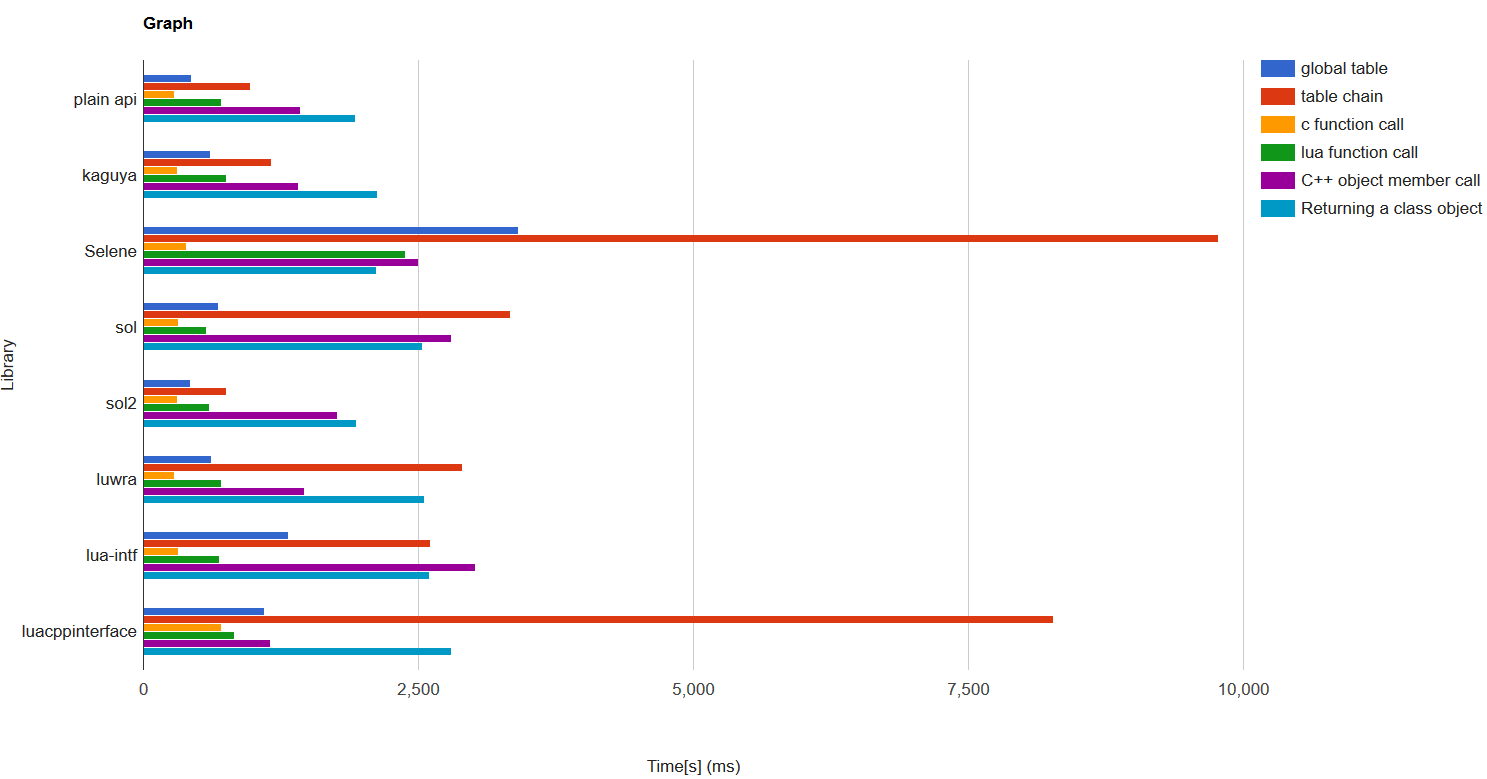
\includegraphics[width=\textwidth]{early-benchmark}
	\centering
	\caption{\textsc{Early benchmarks} created by satoren, developer of Kaguya. Here, various libraries for a given color-coded task are shown, giving the total execution time for 5,000,000 (5 million) iterations. We are doing incredibly well compared to many other libraries and wrappers: \url{http://satoren.github.io/lua_binding_benchmark/}.}
	\label{fig:early-benchmark}
\end{figure*}

\subsubsection{\soltwo{} - Cakewalk}

As this paper is authored by the developer of \soltwo{}, this section will obviously be contain bias. However, it must be said that \soltwo{} provides a number of benefits in API design and efficiency that other libraries do not, and remains one of the most efficient libraries among all categories for the group. 

With fully-featured abstractions such \lstinline|sol::table|; \lstinline|sol::function| and \lstinline|sol::protected_function|; \lstinline|sol::coroutine|; \lstinline|sol::thread|; \lstinline|sol::userdata|; and \lstinline|sol::lightuserdata|, it is fairly clear \soltwo{} covers almost every single specific type that Lua offers with a higher-level covering. Abstractions for the debug framework are missing, and a potential \lstinline|TODO| would be the at least providing enough of an abstraction on top of that for a lua-based stack-trace when the default panic function is called. Its simplicity is proven by the praise that Lua veteran Sean Conner on the Lua mailing list gave \soltwo{} when he was given an example\cite{conman-impressed}. Jason Turner commented during a C++ Now 2016 scripting discussion that he was \href{http://chat.stackoverflow.com/transcript/message/30509197\#30509197}{"super impressed"}.\\

\hfill "For ease of use and performance it's really quite good. I'd say it's the second best scripting option for C++ :wink:" -- Jason "Lefticus" Turner, creator of ChaiScript

\hfill May 16, 2016 \\

Reception on reddit was also overwhelmingly positive\cite{sol2-reddit}. \soltwo{} even attracted users away from other libraries once enough documentation and tutorials existed to demonstrate just how fully featured \href{https://github.com/ThePhD/sol2/issues/36\#issuecomment-199290974}{\soltwo{} is}. Our usertype abstraction is also one of the most terse, going with a key-value style of additions with various wrappers to provide functionality akin to Luabind's properties, Luabind's factory/constructor calls, and read/write only memory from SWIG.

\begin{lstlisting}[caption={\soltwo{} usertype example, performing the same binding for the \lstinline|basic| class as shown with many of the other libraries. Noticeably more terse.}, label={lst:sol-usertype}]
sol::state lua;
lua.new_usertype<basic>("basic",
	"var", &basic::var,
	"get", &basic::get,
	"set", &basic::set
);
\end{lstlisting}

Libraries that have started 2-4 years before \soltwo{} have less stars and less watchers, with \soltwo{} breaking 160 stars with small, steady growth continuing (with the exception of the extremely popular Selene). Additional advertising on the lua mailing list and perhaps a talk about the optimization and implementation of \soltwo{} are in the works. Documentation hosted at ReadTheDocs\cite{readthedocs} has proven immensely useful, allowing users to make simple pull requests to change documentation with automatic updates if they accept. Iris Zheng, a student at Columbia University, was extraordinarily helpful in improving \soltwo{}'s documentation for beginners, making it much easier to get those who were not entirely used to C++ and its many environments to pull the header-only library and get started.

\soltwo{} is Lua-version-agnostic. So long as some form of LuaJIT or Lua 5.1 or above are in place, \soltwo{} will work without problem. This is ensured by tests written under the Catch\cite{catch} framework.

\textbf{Recommendation}: Use \soltwo{}. Issues are gladly accepted at the repository. Turnaround time for responses is less than 24 hours, sometimes with fixes and implementations coming around that fast as well. Development is active and additional performance enhancements are already planned.

\begin{figure*}[ht]
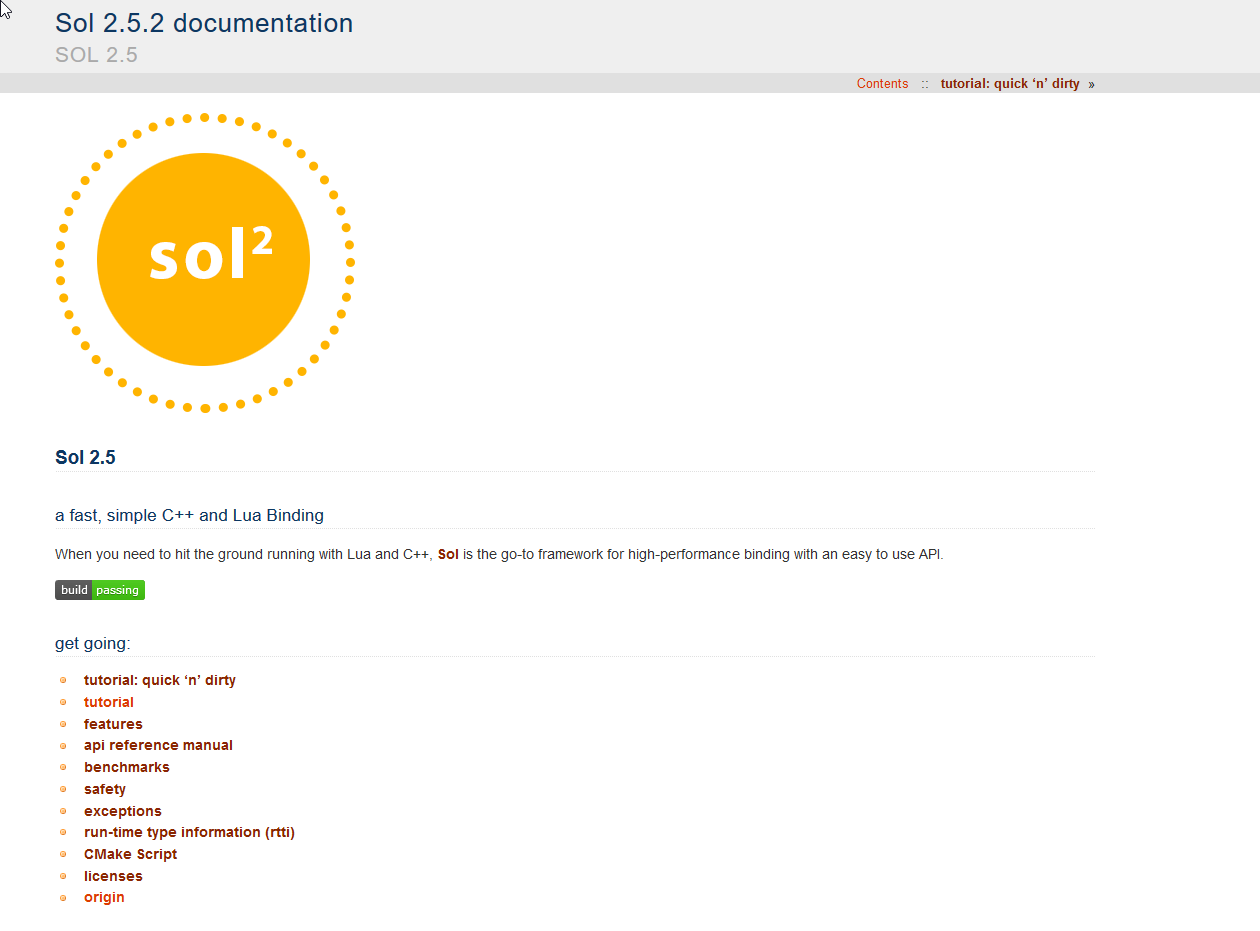
\includegraphics[width=\textwidth]{docs}
\centering
\caption{\textsc{The documentation} of \soltwo{} hosted by ReadTheDocs: \url{http://sol2.readthedocs.io/en/latest/}.}
\label{fig:docs}
\end{figure*}


\subsection{Performance Comparisons}

Aside from satoren's benchmarks (see \cref{fig:early-benchmark}), there is only raw data available at the moment concerning performance of \emph{all} thirteen APIs. The data and benchmarks are available online\footnote{Additional benchmark data that has not yet been massaged into graphs and covers greater detail than the benchmarks shown in this paper are at \url{https://github.com/ThePhD/lua-bench/tree/master/lua - results}. The overall benchmarking code and projects can be found at \url{https://github.com/ThePhD/lua-bench}.}. The additional data needs to be massaged into a clean representation using python's matplotlib from the "lua crunch" project in that repository (pull requests welcome). From both satoren's benchmarks and lua-bench's initial CSV numbers generated from statistical microbenchmarking framework nonius\cite{nonius}, Kaguya, luwra, and \soltwo{} seem to be the most highly performing across all areas, with Selene quite demonstrably being the worst optimized of the group.


\section{Conclusion}

From our analysis of over a dozen wrapper APIs, it is clear that there are really only 2 choices to use when developing in C++ and one needs to reach out for Lua wrapper to help them embed the language in their application/system. Kaguya and \soltwo{} provide the most features, abstractions, and speed to date, with Kaguya filling the niche of compatibility and \soltwo{} filling the niche of heavily featured. Both are efficient and performant enough, even if there is some evidence for \soltwo{} being faster.

The most important part of this project has been learning that \emph{\textbf{documentation is key}}. The reason SLB3 is a pain to use is because the documentation is outdated and sparse, along with the developer dropped off the face of the earth. luacppinterface was equally difficult to grok until looking at its tests to understand how it was used, as well as other individuals who used it. Selene and Kaguya had readme-style, shamelessly quick, code-snippet-examples style documentation that had users up and running in minutes, resulting in a confidence that kept users coming to both wrappers and continuing to use them. Usable, helpful documentation is a premium in the software development world, far more than unit tests or continuous integration build badges.

Creating those docs three months ago from the time of writing (May 2016) was a massive boon. This user friendliness was further compounded by Iris Zheng's help, alongside several Github user's input that truly shaped up a decent tutorial. At one point some of our potential users \emph{thought} that \soltwo{} had more features, but they were not sure because they could not get to our documentation. This proved an important lesson on making sure users got to our documentation, and hosting it on ReadTheDocs helped that happen swiftly. \soltwo{} is ready to change how developers look at scripting language APIs in C++ for a long time to come, and I sincerely hope it becomes the golden standard for Lua inter-operation in C++.

% use section* for acknowledgment
\ifCLASSOPTIONcompsoc
  % The Computer Society usually uses the plural form
  \section*{Acknowledgments}
\else
  % regular IEEE prefers the singular form
  \section*{Acknowledgment}
\fi

A humongous Thank You to: Professor Gail Kaiser to letting the focus of COMS E6156's Topics in Software Engineering be about the use and improvement of \soltwo{}; Ms. Iris Zhang for using, improving, and vetting the documentation; Kevin Brightwell (\href{https://github.com/Nava2}{Nava2}) for Travis CI build improvements; Sean Conner for his help on the Lua Mailing List; the various Github issue openers and contributors for improving documentation, suggesting features, and catching bugs in \soltwo{}; Danny Y. (\href{https://github.com/Rapptz}{Rapptz}) for starting and implementing Sol; and, the \href{http://loungecpp.net/}{\loungecxx{}}.


% trigger a \newpage just before the given reference
% number - used to balance the columns on the last page
% adjust value as needed - may need to be readjusted if
% the document is modified later
%\IEEEtriggeratref{8}
% The "triggered" command can be changed if desired:
%\IEEEtriggercmd{\enlargethispage{-5in}}

% references section

% can use a bibliography generated by BibTeX as a .bbl file
% BibTeX documentation can be easily obtained at:
% http://mirror.ctan.org/biblio/bibtex/contrib/doc/
% The IEEEtran \textsl{}BibTeX style support page is at:
% http://www.michaelshell.org/tex/ieeetran/bibtex/
% argument is your BibTeX string definitions and bibliography database(s)
\bibliography{references/bibliography}
\bibliographystyle{IEEEtran}
%
% <OR> manually copy in the resultant .bbl file
% set second argument of \begin to the number of references
% (used to reserve space for the reference number labels box)
%\begin{thebibliography}{1}
%\end{thebibliography}




% that's all folks
\end{document}


